\chapter{Case Study II: Cellular Networks}
\label{chap:casestudy2}
\section{Prelude}

Cellular networks consume several tens of TWhs (terawatt-hours) of electrical energy worldwide every year~\cite{Oh:Comm:2011}, exacerbating rising ecological concerns. Beyond these concerns, the corresponding cost of electricity makes up a significant proportion of the overall operational cost of a cellular service provider.
In European markets, for example, the electricity cost is
estimated to be around 18\% of the operational costs~\cite{Blume:2010:BLTJ:CellularPower}.
This fraction is even higher in developing regions due to the shortage of grid electricity and the use of small-scale generation powered by diesel fuel. Thus, cellular operators are keen on reducing the power consumption of their networks.

In this chapter, we discuss RED-BL's application to save energy in cellular networks. To this end, we utilize \textit{Base
Transceiver Station (BTS) Power Savings} and \textit{Call
Hand-off} to reduce the BTS power consumption. Using deployment
and traffic data from a cellular provider in a large metropolitan area in a developing region, we show that using RED-BL's optimal solution can save about 10\% in the amount (and cost) of electrical energy.
This translates into millions of dollars in annual savings, just for this one service provider.


This saving in energy consumption is achieved by reducing the power consumption at BTSs, which account for 60\% to 80\% of a cellular network's total power consumption~\cite{Oh:Comm:2011,Louhi:2007:BTSPower:INTELEC,Peng:2011:BTSSaving:Mobicom}, by making them more energy proportional.
Figure~\ref{fig:workload-variation} shows the normalized load of consumer traffic at two neighboring BTSs in our dataset.
Observe that while the traffic load peaks for a short period of time, it mostly stays at a fraction of its peak\footnote{Operational cellular networks have been widely observed to exhibit traffic load variations both over time and space \cite{Peng:2011:BTSSaving:Mobicom}.}.

However, the radio circuitry at BTSs is provisioned in accordance with the peak load.
This radio circuitry lacks energy proportionality, i.e., its power consumption does not scale in proportion to the traffic load.
As a result, a BTS also lacks energy proportionality and consumes power at about the same level as it would at the peak load~\cite{Peng:2011:BTSSaving:Mobicom}. This leads to wasted energy, which RED-BL aims to reduce---by varying the power consumption at a BTS in accordance with its traffic load.

\begin{figure}[t]
\centering
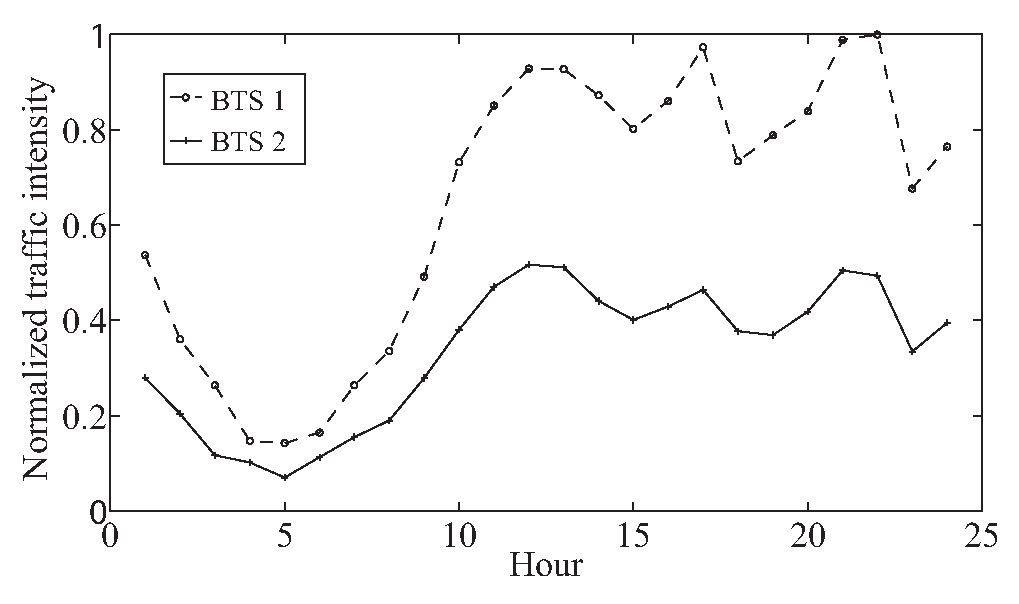
\includegraphics[width=0.8\textwidth]{pics/ilyas1.eps}
\caption{Traffic load variations at two neighboring BTSs during a single day from our dataset. For most of the day, the instantaneous load is a fraction of the peak traffic load.}
\label{fig:workload-variation}
\end{figure}


If the instantaneous power consumed at a BTS can be made proportional to the instantaneous
workload, savings in power consumption will ensue.
For the provider data available to us, a fully energy proportional BTS subsystem of a cellular network would save between $44\%$$-$$52\%$ of electrical energy depending on the BTS model.
Thus, there exists potential to save electricity cost in a cellular network by reducing the energy consumption at low workloads.
RED-BL exploits this potential in two ways: (i) \textbf{Resource pruning}: shutting down part of the radio circuitry, and (ii) \textbf{workload relocation}: rerouting calls from one BTS to a nearby BTS.

 
Coarse-grained energy proportionality in BTSs may be achieved in one of the following two ways:
\begin{itemize}
\item BTSs may be turned off when traffic is low and turned on later when traffic load
increases~\cite{Oh:TWC:2013,6503647,Oh:Globecom:2010,5208045,Oh:Comm:2011,marsan:wgreen:2008}.
However, operators are often reluctant to switch on/off entire BTSs due to coverage and equipment lifetime concerns.
\item \textit{Frequency dimming}~\cite{Tipper:Dimming:Globecom:2010} proposes to turn off a fraction of
the radio circuitry when traffic is low, such that the traffic may be handled by the circuitry that stays on.
Most vendors' BTSs support such a feature, which we term as \textit{BTS power savings} in this paper.
Our conversations with cellular operators reveal that they regularly use this feature. We use this feature as the RP strategy in the RED-BL formulation.
\end{itemize}

Traffic traces collected from a large network operator indicate that if some calls are handed off between
neighboring BTSs, the number of BTSs that can be put in BTS power savings mode can be increased.
Thus, we propose to hand-off calls between neighboring BTSs, without making a negative
impact on the network quality of service, such that the \textit{BTS power savings} can be applied to a
maximal number of base stations throughout the cellular network. In comparison to uncoordinated \textit{BTS power savings}, as used in current cellular network deployments, RED-BL
offers additional power savings as it may allow a larger number of radio circuits to be deactivated.

The underlying assumption in RED-BL is that calls can be handed off to neighboring BTSs
without being dropped and without exceeding their traffic capacity. This is possible because (a) traffic load in cellular networks exhibits significant variation over time and space and (b)
most callers often receive sufficiently strong signal from \emph{several} nearby
BTSs~\cite{Peng:2011:BTSSaving:Mobicom,lowcarb:2013:globecom}.
This coverage diversity is evident in Figure~\ref{fig:btscdf}, which shows the CDF of the number of BTSs available to an end-user in our dataset of live traffic.
Observe that the results show that about half of the callers have 3 or more candidate BTSs available at all times
Thus, some calls may be handed off from one BTS to a nearby BTS in order to increase energy savings over those
possible through BTS power savings alone.
\begin{figure}[h!]
\centering
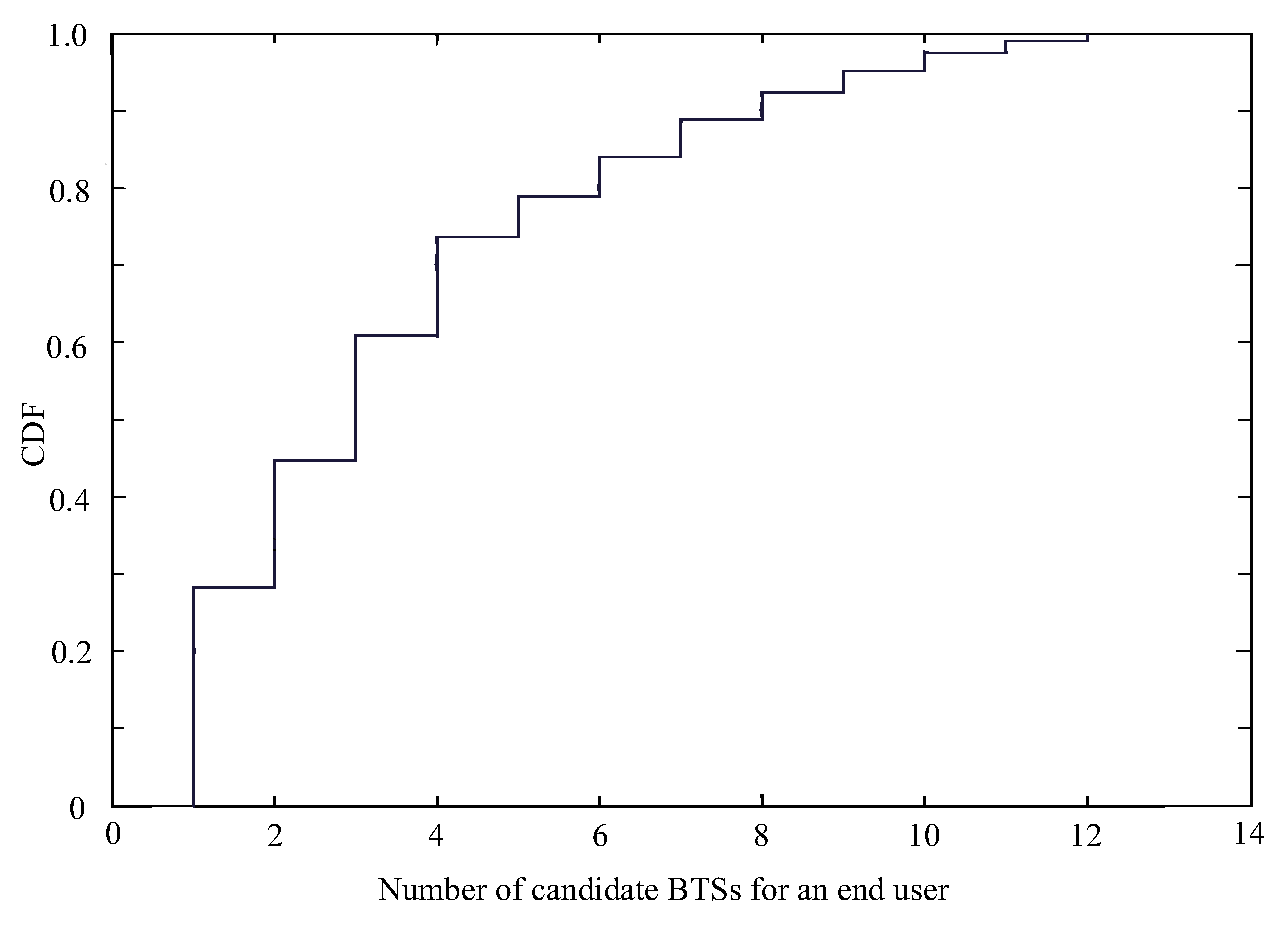
\includegraphics[width=0.8\textwidth]{pics/ilyas2.eps}
\caption{Cumulative distribution function (CDF) of the number of potential serving BTSs for a call in our dataset (large metropolitan area).}
\label{fig:btscdf}
\end{figure}

During low traffic periods, network operators often use a feature available in most vendor's equipment that deactivates TRX circuits at locations that
serve very few customers. Huawei calls this feature \textit{TRX shutdown} while Ericsson calls it \textit{BTS power savings}. We use the latter term generically in this paper. Turning off one TRX cuts down BTS power consumption anywhere from $20W$
to $100W$, depending upon the frequency band (900 or 1800) and
deployed
equipment~\cite{Lorincz:BTS-Measure:Sensors:2012,flexibsc}.
Thus, scaling a ``6+6+6'' to a ``2+2+2'' configuration, by deactivating 12
TRXs will result in a saving of
240W to 1200W on a single site.

\subsection{Motivating example}

\begin{figure}
\centering
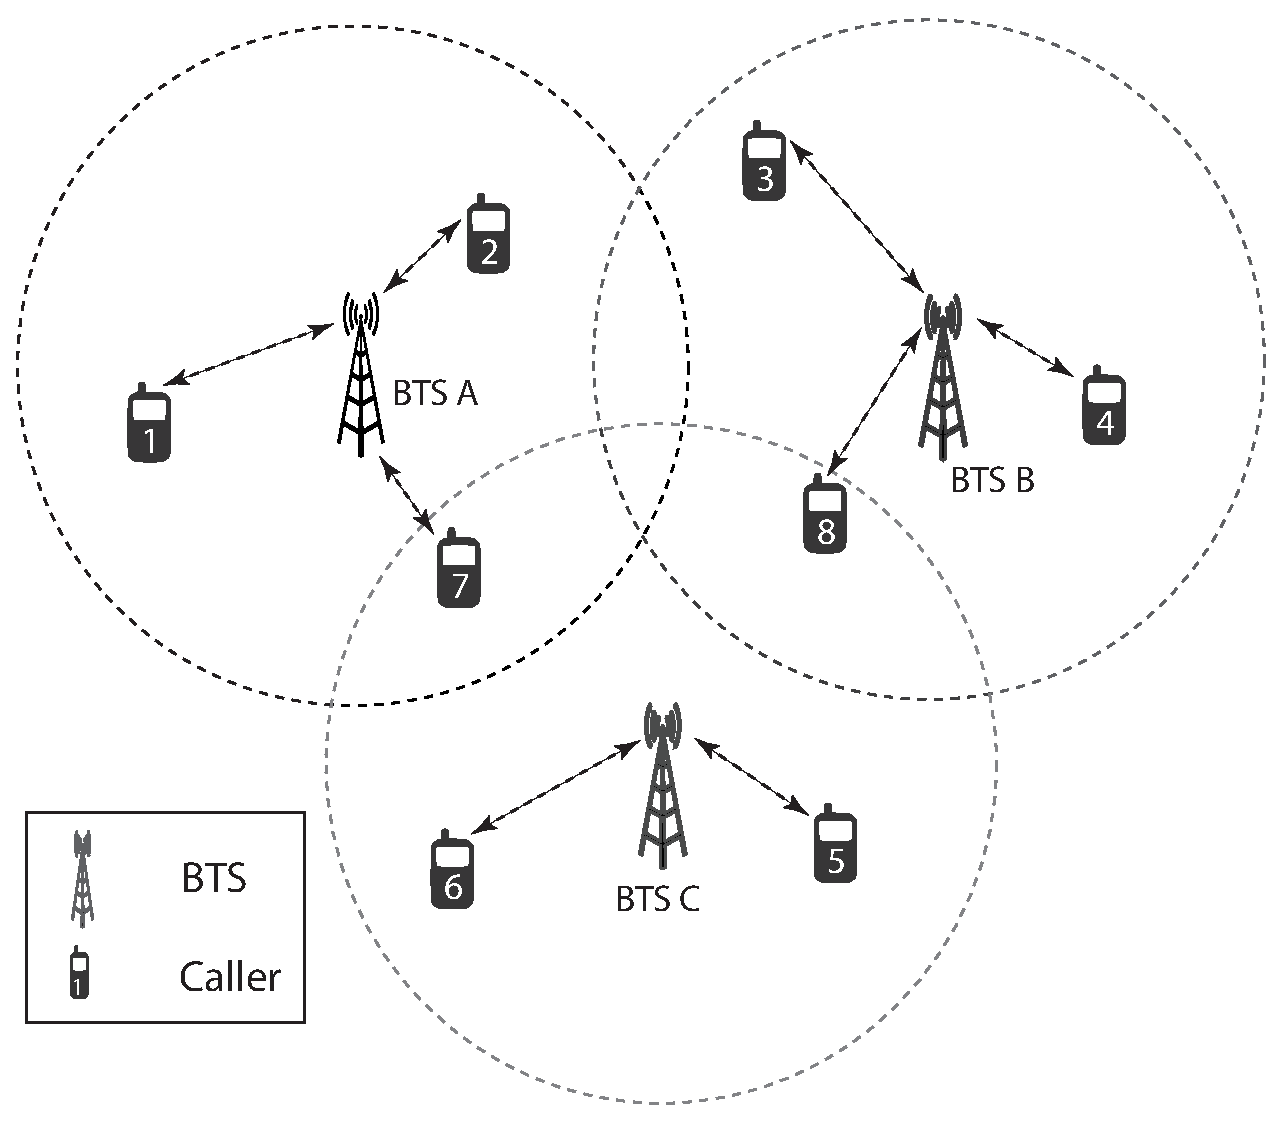
\includegraphics[width=0.6\textwidth]{pics/ilyas3.eps}
\caption{The scenario for the motivating example. Three BTSs (A, B and C) are shown along with eight active calls. Each call is handled by the BTS from which it receives the strongest signal (the default in GSM networks). The serving BTS for each call is shown using arrows. If the power savings mode can be enabled at a BTS that has up to two active calls, then only BTS C can be put in the power savings mode. However, if calls 7 and 8 were handed off to BTS C, both BTS A and B can be put into the power savings mode, thereby resulting in greater energy savings.}
\label{fig:illustrationall}
\end{figure}

\begin{table}
\centering
\begin{tabular}{|c|c|c|c|c|}
\hline
Scheme & \multicolumn{3}{|c|} {Calls being handled by BTSs} & BTSs in power \\
\cline{2-4} \ & A & B & C & saving mode \\
\hline Default & 1, 2, 7 & 3, 4, 8 & 5, 6 & None \\
\hline Power saving & 1, 2, 7 & 3, 4, 8 & 5, 6 & C \\
\hline RED-BL & 1, 2 & 3, 4 & 5 -- 8 & A, B\\
\hline
\end{tabular}
\vspace{+0.1in}
\caption{A comparison of schemes for BTS power savings}
\label{tab:example}
\end{table}

To illustrate the working principle of RED-BL, we consider an example deployment consisting of three BTSs serving eight calls in neighboring cells as shown in Figure~\ref{fig:illustrationall}.
By default, each call is served by the BTS from which the mobile station receives the strongest signal. Assume that each BTS may handle up to six simultaneous calls and that the power-saving threshold is two calls, i.e., a BTS serving up to two calls may be put into power-saving mode.

The first row in Table~\ref{tab:example} indicates that under default call association, no BTS in the example deployment of Figure~\ref{fig:illustrationall} is placed in power saving mode.
With this default call association, the operator may still save some electrical energy by activating the power saving mode on BTS C (second row in Table~\ref{tab:example}).
Additional energy savings are possible by deploying the optimal solution to RED-BL, which hands off calls 7 and 8 to BTS C and enables power saving mode on two BTSs (A and B), as shown in the third row in Table~\ref{tab:example}.


This example shows that the current practice of enabling power savings mode based on traffic conditions that are local to a BTS can result in sub-optimal energy savings.
RED-BL achieves greater energy savings by jointly using call hand-off and BTS power savings.

\section{Related work}
\label{sec:related}

The power consumption of a BTS depends on a number of factors. A BTS's power consumption increases with the number of TRXs. The frequency band, modulation scheme and operating conditions also influence a BTS's power consumption~\cite{hasan:2011:green}. Accordingly, various researchers have attacked the BTS energy efficiency improvement problem from various angles.

For a given traffic load, the power consumption of a BTS may be reduced by using more energy efficient designs for the components such as TRXs. One such technique is to use switch mode power amplifiers instead of linear analogue power amplifiers~\cite{ertl:2002:analysis,mccune:2005:high,yoo:2001:common,grebennikov:2012:switchmode} or other architectural improvements~\cite{amanna:2010:green,claussen:2008:effects}. In~\cite{claussen:2008:effects}, the authors showed that the energy efficiency of macro-cell based deployments deteriorates with increasing demand for higher data rate services and proposed that a hybrid deployment of residential pico cells and macro-cells be used instead. They showed that this can result in a 60\% reduction in energy consumption. In contrast to~\cite{claussen:2008:effects}, our focus is on making incremental changes to a deployed network that is based predominantly on macro-cells to reduce the energy consumption.
 
In~\cite{Peng:2011:BTSSaving:Mobicom}, the authors proposed that when the traffic in an area being served is low, the serving BTS may be completely turned off to save power. Later, when the traffic volume rises, such BTS may be turned on again. To avoid lack of coverage when a BTS is turned off, its neighboring BTSs must, however, increase their transmit power.
Similar proposals are also reported in~\cite{Oh:TWC:2013,6503647,Oh:Globecom:2010,5208045,Oh:Comm:2011,marsan:wgreen:2008}. In~\cite{marsan:2011:energy}, Marsan et al. considered wireless Internet access in an area covered by multiple operators. They proposed that under high traffic conditions, all networks should operate but as the traffic drops, networks could be progressively turned off to save energy. Our conversations with cellular operators in Pakistan indicate that they are reluctant to turn off entire BTSs due to reduced expected lifetime of the installed electronic equipment.

Several centralized as well as distributed algorithms for placing maximal number of BTSs in sleep mode or turning them off during low traffic load have been proposed recently. For instance, it was proposed in~\cite{samdanis:2010:self,samdanis:2010:dynamic} to group nearby BTSs in an LTE network into energy partitions and then hand-off traffic out of lightly loaded BTSs to put them into sleep or turn them off. Also in the context of LTE networks, Viering et al. proposed an algorithm that adjusts transmission power levels for BTSs in response to traffic load variations with small changes to the coverage area.

\textit{Frequency dimming}~\cite{Tipper:Dimming:Globecom:2010} proposes to turn off some TRXs on a BTS when the traffic is low. RED-BL goes beyond frequency dimming --- it reroutes the calls and can potentially enable power savings mode on a larger number of BTSs.
Coarse estimates of the energy saving potential of TRX deactivation were presented
in~\cite{Blume:2010:BLTJ:CellularPower}.
In contrast, we use site locations and real traffic traces from a large cellular network with more than 13 million subscribers to run a simulation study assessing the benefits of dynamic equipment scaling coupled
with call hand-offs. Note that BTS power saving represents RP in the RED-BL framework whereas call handoff represents WR.

Some prior work that has used call hand-off to optimize power consumption include~\cite{Dufkova:2010:EW,zhou:2009:mobicom,yang:2013:TVT}. In~\cite{Dufkova:2010:EW}, the authors determined the optimal association between mobile stations and base station in an LTE network to minimize BTS power consumption while considering only data traffic. In Pakistan, and many developing countries, voice traffic is still quite dominant in cellular networks. Data traffic and text messages are considered low-priority traffic. Hence, in our context, considering data traffic to minimize power consumption is not useful. In~\cite{zhou:2009:mobicom}, the authors used relay stations to hand off calls to other BTSs in order to minimize power consumption. The use of relay stations within cellular networks in developing countries is rare, hence we do not consider their use in this work. 

There exists a large body of work on solutions to constrained resource optimization problem, like the one we formulate for RED-BL. For example, such problems have been addressed in the context of data centers~\cite{Jeyarani:2012:DIA:2148243.2148374,serverEnergy,Mazzucco:Maximizing:2011:CoRR,Oh:2011:ECS:2170444.2170458,Chase:2001:MES:502059.502045}, scheduling in compute clusters~\cite{AlDaoud2012745}, System on Chip (SOC)~\cite{Fang:2011:COP:1995896.1995940}, electric power systems and smart grids~\cite{Javed:2008:ULP:1485753.1485792,Logenthiran2011138,Celli:2001:PICA,FahadJavedAdOpt.SASO.2009.26}, WiFi access points~\cite{Marsan:2010:SAM:1791314.1791340}, wide area networks~\cite{Cavdar:2011:ECOC} and high performance computing~\cite{Lee:ServerConsolidation:2011:Globecom,Pinheiro01loadbalancing,Yao:DCPowerReduction:2012:INFOCOM,Herodotou:Starfish:2011:CIDR,Herodotou:2011:NOS:2038916.2038934,Aikema:ElecCostHPC:2011:ISSST}.

\section{Instantiating the generalized optimization formulation} %Derive the objective function and constraints. Clearly outline the assumptions that we've made about the geo-diverse data centers.
\label{sec:case2:instantiate}
The RED-BL optimization formulation minimizes the sum of state and transition costs for a network over a sequence of consecutive intervals in a planning window. The state cost for a particular interval is the sum of electricity cost incurred at all BTSs in the network. In order to compute the state cost, we will first derive a mathematical model for electricity consumption at a single BTS. Then, we will generalize it to a multi-BTS cellular network setting to represent the state cost for a single interval. The transition cost would be the cost of electricity incurred in activating or deactivating TRXs. Our conversations with network operators reveal that transitions into and out of BTS power saving mode do not consume a noticeable amount of power. These state transitions are reasonably fast in contrast to the delayed convergence due to transitions in the geo-diverse data center scenario. The same is confirmed from the results in~\cite{marsan:2011:ICC}. The transition costs in the RED-BL formulation as applied to a cellular networks may, therefore, be ignored.

If $\delta$ is the traffic capacity of a single TRX, then the traffic handling capacity of BTS with $r$ TRXs is $r\delta$. If $x_i$ is the number of calls currently in progress at BTS $i$, and the power consumed by the BTS under no load and full load is $P_{min}$ and $P_{max}$, respectively, then the instantaneous BTS power consumption at the BTS\footnote{In the following discussion, when we refer to BTS power consumption, the implication is the component of BTS power consumption due to TRXs only. Since TRXs account for a large fraction of BTS power consumption~\cite{Lorincz:BTS-Measure:Sensors:2012}, minimizing TRX power consumption will reduce BTS power consumption.}, $P_i$, approximated as an affine function of its traffic load~\cite{Peng:2011:BTSSaving:Mobicom}, is given by
\begin{align}
P_i = P_{min} + x_i(P_{max}-P_{min})/r\delta\label{eq:btspower}
\end{align}

If a TRX's no-load power consumption is $\gamma$ (its value depends on the equipment type~\cite{Lorincz:BTS-Measure:Sensors:2012,flexibsc}), then $P_{min}=a\gamma$, where $a$ is the number of active TRXs.
Thus, by scaling the number of active TRXs in response to traffic volume changes, BTS power consumption may be reduced.
For example, if the traffic volume at a BTS falls below a power-saving threshold $r\delta/2$, then half of the TRXs may be turned off.
As a result, the BTS will transition to the low-power mode whereby the power consumption profile drops by an amount $r\gamma/2$ as shown in Figure~\ref{fig:powermodel1}. The slope of the power consumption profile remains the same whether or not the BTS is operating in low-power mode. 

If the BTS is switched into low-power mode as soon as traffic falls below $r\delta/2$, then short time scale variations in traffic might cause a TRX to turn on/off rapidly. Since this may be detrimental to a TRX's lifetime, low-power mode is activated only when traffic reaches threshold $r\delta/2-\epsilon$. Here, $\epsilon$ is a parameter which may be set equal to 0 to achieve an aggressive power saving strategy of turning off a TRX as soon as opportunity presents itself. On the other extreme, $\epsilon$ may be set equal to $r\delta/2$ in which case a TRX is never turned off. These two extremes relate to a trade
off between equipment lifetime and energy savings.

Instead of the all-or-half approach of Figure~\ref{fig:powermodel1}, power-saving may also be applied in a more granular way, such as that shown in Figure~\ref{fig:powermodel2}, whereby one-third of the TRX may be switched on/off independently in response to current traffic volume. In general, the number of granular steps in the power-saving strategy is limited by the number of TRXs installed on a BTS.

\begin{figure}
\centering
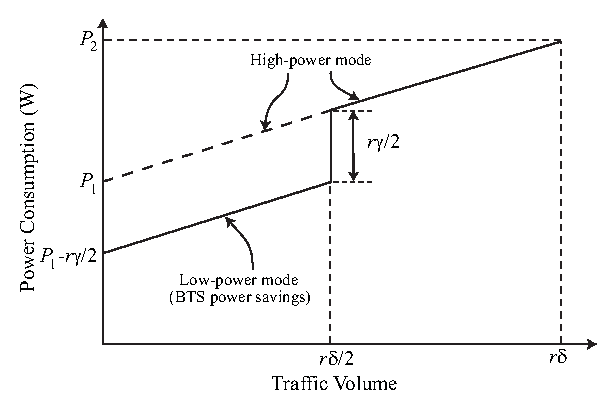
\includegraphics[width=0.7\textwidth]{pics/ilyas4a.eps}

\caption{Two-state power consumption model for a BTS with $r$ TRXs. Low-power (BTS power savings) mode is optional and kicks in at low loads.}
\label{fig:powermodel1}
\end{figure}
\begin{figure}
\centering
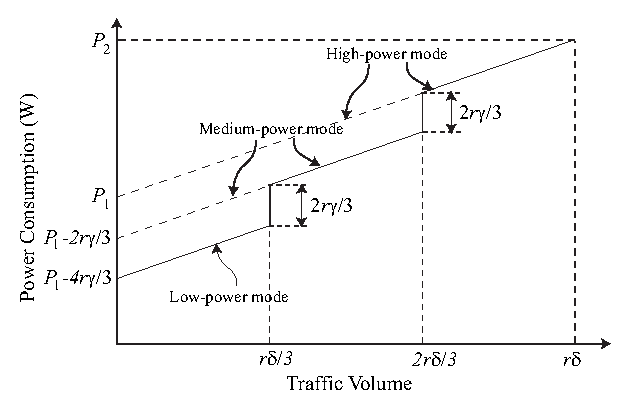
\includegraphics[width=0.8\textwidth]{pics/ilyas4b.eps}
\caption{Three-state power consumption model for a BTS with $r$ TRXs. BTS power savings is applied in a more granular way than the model of Figure~\ref{fig:powermodel1}.}
\label{fig:powermodel2}
\end{figure}

\subsection{Multi-BTS cellular setting}
Since BTS power consumption is an additive function of the number of active TRXs, to minimize the power consumption over the network, we must minimize the total number of active TRXs.  Consider a cellular network consisting of $m$ BTSs and $n$ callers. 
Let $c_{i,j}$ be a binary variable which is equal to one if caller $i$ \textit{can be} served through BTS $j$ and zero otherwise.
Also, let $w_{i,j}$ be a binary variable which is equal to one if caller $i$ \textit{is} served through BTS $j$ and zero otherwise. Suppose that on a particular BTS, we may independently turn on/off a block of $\beta$ TRXs at a time.

Our conversations with network operators reveal that the transition costs resulting from activating or deactivating TRXs using BTS power saving feature of the BTSs is negligible. Thus, the $T(.)$ part of equation~\ref{eq:genobjective} may be approximated as zero. According to equation~\ref{eq:btspower}, the state cost part, $C(.)$, from equation~\ref{eq:genobjective} is a linearly increasing function of the total number of TRXs in the network. If $y_j$ is the number of active TRX blocks at BTS $j$, then the RED-BL optimization problem may be given as: 
\begin{align}
\textit{minimize} \quad \sum_{j=1}^{m} y_j
\end{align}
subject to the following constraints: 
\begin{align}
& \sum_{j=1}^m w_{i,j} = 1 \qquad \forall i \label{eq:handleall}\\
& w_{i,j} \leq c_{i,j} \qquad \forall i, j \label{eq:compatible}\\
& \delta \beta y_j - \alpha - \sum_{i=1}^nw_{i,j} \geq \epsilon \label{eq:margin} \\
& 1 \leq y_j \leq r / \beta \qquad (y_j \in \mathbb{N}) \qquad \forall j \label{eq:x}
\end{align}
The first constraint (Eq. \ref{eq:handleall}) ensures that every call is served by exactly one BTS. The second constraint (Eq. \ref{eq:compatible}) ensures that a call is served by a BTS that \textit{can} serve it, thereby securing the uplink and downlink transmit power budget.
The third constraint (Eq. \ref{eq:margin}) ensures that the number of active TRXs is large enough such that there is a residual call capacity for at least $\epsilon$ more calls\footnote{A number of logical channels are reserved for control purposes in each sector. Here, $\alpha$ is the number of control channels per BTS}.
The fourth constraint (Eq. \ref{eq:x}) specifies the range of values that $y_j$ may take.

The granularity of applying power-saving is determined in the above optimization formulation through the value of $\beta$. For instance, if $\beta$ equals 1, then each TRX may be independently turned on/off. Similarly, if $\beta$ equals $r/2$, the problem reduces to the two-step model of Figure.~\ref{fig:powermodel1}. Setting $\beta$ equal to $r/3$ results in the three-step model of Figure.~\ref{fig:powermodel2}.


\subsection{Problem complexity}
\label{subsec:lccomplexity}
In this section, we develop a proof of NP-Hardness of the energy cost optimization using coordinated WR and RP as applied to cellular networks\footnote{This proof was done through personal communication with Dr. Mudassir Shabir}. For this proof, we define the problem as:
\medskip

\noindent
\textbf{Problem Name:} RED-BL\\
\textbf{Input:}
\begin{itemize}
\item A set of callers $C$
\item A set of BTSs $B$
\item Scalar values $P_1$, $P_2$, $\delta$, $\gamma$, $t_{\max}$
\end{itemize}
\textbf{Output:} An assignment of each caller to exactly one BTS that minimizes the cost as given in equation X.

We also define the modified dominating set problem (MDS) as follows:
\medskip

\noindent
\textbf{Problem Name:} Modified Dominating Set\\
\textbf{Input:} A bipartite graph $G=\{E,V\}$ with sets of vertices $J$, $K$ such that every edge in $E$ connects a vertex in $J$ to a vertex in $K$.\\
\textbf{Output:} A minimum cardinality set of vertices belonging to $J$ that cover every vertex in $K$.

We claim that we can use RED-BL to solve MDS. If we set $\delta$ to 0 and $P_1$ to some non-zero value for RED-BL, then there is a set-up cost on each BTS, i.e., a fixed cost of $P_1$ is incurred for the first call on each BTS. Hence, in this case, the optimal solution to RED-BL will use the fewest number of BTSs to handle all calls. Therefore, if we determine the optimal solution to RED-BL as follows:
\begin{itemize}
\item Set $C$ equal to the vertices in $K$
\item Set $B$ equal to the vertices in $J$
\item Assign $P_1$ some positive value greater than zero
\item Assign $P_2$ some value greater than $P_1$
\item Assign $\gamma$ some positive value greater than zero
\item Set $\delta$ equal to zero
\end{itemize}

then the optimal solution to RED-BL will solve MDS, i.e., use the fewest number of vertices in $J$ to cover all vertices in $K$.

Now, consider the minimum dominating set problem (DS).
\medskip

\noindent
\textbf{Problem Name:} Minimum Dominating Set\\
\textbf{Input:} A graph $G=\{E,V\}$\\
\textbf{Output:} A minimum cardinality subset $D$ of $V$ such that every vertex not in $D$ is adjacent to at least one vertex in $D$

We can solve DS using MDS as follows:
\IncMargin{1em}
\LinesNumbered
\begin{algorithm}
\SetKwData{Left}{left}\SetKwData{This}{this}\SetKwData{Up}{up}
\SetKwFunction{Union}{Union}\SetKwFunction{FindCompress}{FindCompress}
\SetKwInOut{Input}{input}\SetKwInOut{Output}{output}
\Input{A graph $G=\{E,V\}$}
\Output{A minimum cardinality subset $D$ of $V$ such that every vertex not in $D$ is adjacent to at least one vertex in $D$}
 $V_1 = V$\;
 $V_2 = V$\;
 $V^{\prime} = V_1 \cup V_2$\;
 $E_1 = \{(u, v): u \in V_1, v \in V_2$ if $(u, v) \in E$ or $u = v\}$\;
 MDS($V^{\prime}$, $E_1$)\;
\caption{Solving DS using MDS}
\label{algo:proof}
\end{algorithm}
\DecMargin{1em}

We first create two copies of the set of vertices in $G$, named $V_1$ and $V_2$ and add them to set $V^{\prime}$. We also create a set of edges $E_1$ as follows. If there is an edge between vertices $u$ and $v$ in graph $G$, then we add an edge from vertex $u$ in $V_1$ to vertex $v$ in $V_2$. Furthermore, we also add an edge between each vertex $u$ in $V_1$ to vertex $u$ in $V_2$. This results in a bipartite graph $G^{\prime}={V^{\prime}, E_1}$ where every edge in $E_1$ connects a vertex in subset $V_1$ of $V^{\prime}$ to a vertex in subset $V_2$ of $V^{\prime}$.

Invoking MDS on $G^{\prime}$ finds the minimum number of vertices in $V_1$ that cover every vertex in $V_2$. Since $V_1$ and $V_2$ are essentially the same vertices, MDS finds the minimum cardinality set of vertices in $V$ to which all other vertices are connected. Thus, MDS solves DS. It is well know that DS is NP-Hard~\cite{Liedloff:2008:FDS:1390853.1390871}. Since the optimal solution to RED-BL can solve DS, by reduction the former is NP-Hard as well.

\subsection{Heuristic solution to RED-BL for cellular networks}
\label{subsec:heuristics} Even though the energy cost optimization problem using WR and RP is NP-Hard for cellular networks, for a 26 site dataset that we collected from a live cellular network, we were able to find the RED-BL optimal solution within a few seconds.
However, for an entire cellular network, optimally solving RED-BL becomes computationally infeasible.
We propose two ways to handle this intractability. First, the entire network can be divided into several smaller regions and RED-BL can be applied to each region independently.
Second, a heuristic solution to RED-BL, such as the one given in Algorithm~\ref{algo:heur2}, may be applied to the entire network.

The pseudo code for our proposed heuristic is given in Algorithm~\ref{algo:heur2}. In the first iteration of the outer loop (lines 1 through 29), our heuristic divides the set of BTSs into two sets.
Set $B_1$ consists of those BTSs that have traffic volume greater than $(r-\beta)\delta$. The set $B_2$ consists of all other BTSs.
The heuristic algorithm picks a BTS from the set $B_1$ uniformly at random.
It then attempts to move this BTS to set $B_2$ (lines 23--26) by handing off some calls to other BTSs in $B_2$ without exceeding the power-saving threshold\footnote{Note that if the traffic exceeds the power-saving threshold for one or more BTSs in the set $B_2$ after the calls are handed off, it would cause BTSs to move to set $B_1$, which is undesirable.} (lines 12--19).
In the end, blocks of $\beta$ TRXs may be turned off on all members of $B_2$ (line 28).
Further iterations of the outer loop attempt to turn off more blocks of $\beta$ TRXs in a similar manner.

%\begin{comment}
%To solve the three-state Low-Carb problem we invoke our heuristic twice. In the first invocation, we assign to $B_1$ all BTSs that have traffic above threshold $\delta_2$, and all others BTSs are assigned to $B_2$. In the second invocation of the heuristic, we assign all BTSs that have traffic above $\delta_1$ to set $B_1$ and all other BTSs to $B_2$. At the end of the second invocation, those BTSs that have traffic above $\delta_1$ but below $\delta_2$ are placed in the medium-power mode while those with traffic below the $\delta_1$ threshold are placed in the low-power mode. As for the two-state version of the problem, this process may be repeated multiple times to increase the probability of finding a near-optimal solution.
%\end{comment}
Our heuristic is a O($rm^2n/\beta$) randomized algorithm, which is not guaranteed to find the optimal solution. However, a high quality solution is likely to be obtained if the best solution is picked from amongst several invocations of the algorithm.

\IncMargin{1em}
\LinesNumbered
\begin{algorithm}
\SetKwData{Left}{left}\SetKwData{This}{this}\SetKwData{Up}{up}
\SetKwFunction{Union}{Union}\SetKwFunction{FindCompress}{FindCompress}
\SetKwInOut{Input}{input}\SetKwInOut{Output}{output}
\Input{$B$ (the set of BTSs) = \{$b_1, b_2, ..., b_m$\},\\$n$ (the number of calls),\\$W$ (call association) = \{$w_i^j | 1 \le i \le n,$\\ \quad $1 \le j \le m$\},\\$C$ (Adjacency matrix) = \{$c_{i,j}$ = 1 if $c_i$ can \\\quad be served through $b_j$, $0$ otherwise\}}
\Output{A new and potentially more energy efficient mapping of calls to BTSs}
\For{$k := 1$ to $r/\beta$}{
 $B_2$ = $\{b_j | \sum\limits_{i=1}^{n}w_i^j<k\delta\}$\;
 $B_1$ =  random\_shuffle($B - B_2$)\;
 \ForAll{$b_j \in B_1$}{
 	$a = \sum\limits_{i=1}^{n}w_i^j - \delta$\;
 	$d = 1$\;
 	$s = 0$\;
	\While{$d < n$ AND $s \le a$}{
 		\If{$w_d^j=1$}{
 			$e = 1$\;
 			$m = 0$\;
 			\While{$e \le m$ AND $m = 0$}{
 				\If{$e \in B_2$ AND $c_{d,e}=1$}{ 	
 					$w_d^e = 1$\;
 					$w_d^j = 0$\;
 					$s = s + 1$\;
 				}
 				$e = e + 1$\;
 			}
 		$d = d + 1$\;
 	}
 	}
	\If{$\sum\limits_{i=1}^{n}w_i^j < (r-k\beta)\delta$}{
		$B_1$ = $B_1 - \{b_j\}$\;
		$B_2$ = $B_2 + \{b_j\}$\;
		}
 }
	
		Deactivate $\beta$ TRXs on all BTSs $\in B_2$\;
}
\caption{Energy-saving heuristic}
\label{algo:heur2}
\end{algorithm}
\DecMargin{1em}

\section{Experimental setup}
Our dataset is obtained from a cluster of 26 BTSs operated by a large network operator with more than 7000 sites. These 26 sites are spread over a $31.25$\,$km^2$ urban terrain. We obtained each site's coverage prediction using a tool called Forsk Atoll~\cite{atoll} which is quite popular in the cellular network operators community. Using this BTS coverage prediction and a caller's location, we can determine the candidate set of BTSs for the corresponding call (the $c_i^j$ parameters). 

Also available to us are the hourly cumulative traffic, in Erlang, for each of the sites, spanning two consecutive weekdays. The traffic remained remarkably similar across both days for each site. We have, therefore, only used one day's traffic data in our experiments.

Using the above datasets, we conducted a set of simulation experiments mimicking a 24-hour operation of a cellular network comprising 26 cells.
Each experiment is a discrete event simulation of the arrival and placement of calls.
Under the assumption of Poisson call arrivals and given the hourly traffic intensity (in Erlang) for each BTS, we use Little's law to determine the corresponding Poisson call arrival rate.
Our simulator schedules call arrivals for \emph{each} BTS according to this Poisson call arrival process.
For each call, its departure event is also scheduled based on an exponential distribution of call durations with a mean of $180$ seconds~\cite{Gerla:1995:MMM:276418.276421}.

The location where each call originates in a cell is uniformly distributed over the corresponding BTS's coverage area. Based on the randomly picked location at which a particular call originates, the entries $c_{i,j}$ are determined such that $c_{i,j}$ = 1 if call $i$ is within service range of BTS $j$.

To mimic present day practices in operational networks, our simulator associates each call to the BTS from which the received signal is strongest. Using this call-BTS association, a time series of traffic load for each BTS is calculated, which determines the power consumption profile for each BTS. Integrating the power consumption time series for each BTS gives its energy consumption over a 24 hour period. Summing the energy consumption for all BTSs gives the network's total energy consumption. This number represents a baseline for assessing the performance of the energy efficiency improvement techniques that we investigate.

Iterating over the traffic load time series for each BTS, our simulator places those BTSs that have sufficiently low traffic into power-saving mode. Using the power consumption functions given in equation~\ref{eq:btspower}, our simulator calculates the energy consumption for the network over a 24 hour period when BTS power-saving is applied.

During the simulation, at a configurable frequency, we also invoke the solver for RED-BL optimization formulation using the current call traffic. We thus determine the energy consumption for the network over a 24 hour period when call hand off and BTS power saving are applied in a coordinated fashion.

If the solution to RED-BL formulation is determined and deployed very frequently, the network will remain in an optimal state most of the time. Therefore, an aggressive re-optimization scheme will enable greater energy savings. In order to study how the energy savings scale with re-optimization frequency, we experimented with a range of intervals between successive optimizations, ranging from a minute to an hour.

\subsection{Site characteristics}
\label{subsec:sitetypes} All sites in our dataset had three sectors, each equipped with 6 TRXs. The maximum number of simultaneous calls for each site is 132~\footnote{Each TRX's frequency is shared in time-domain  by 8 calls for  a total of $3\times6\times8=144$ channels. Four channels in each sector were reserved for control and broadcast purposes, resulting in 132 channels available for voice calls. The half-rate codec feature of GSM standard can be used to handle greater traffic volume, but we do not consider it in the present work in favor of model simplicity.}. 

The BTS power consumption model parameters may vary from one equipment to another. In this thesis, we use three different sets of model parameters as listed in table~\ref{tab:models}. We now describe the sources and methods from which we obtained these models.

\subsubsection{Model 1}
\label{subsubsec:model1}For the first model, we have used $1.5$\,kW as the maximum power consumption~\cite{mbakwe:btshybribpower:2011:necec}, a $20$\,W per TRX saving when scaling the BTS down~\cite{flexibsc} and a $5$\,\% variation in power consumption between no-load and full-load~\cite{Peng:2011:BTSSaving:Mobicom}.

\subsubsection{Model 2}
\label{subsubsec:model2} Lorincz et al. reported the single sector DC power consumption for a GSM 900 BTS~\cite{Lorincz:BTS-Measure:Sensors:2012}. The sector under consideration had 7 TRXs, as opposed to 6 TRXs in our case. To approximate the DC power consumption for a site with 3 sectors, each with 6 TRXs, we scaled the power consumption by a factor of $3\times6/7$. The DC power consumption does not include the AC power consumed in the power supply units and in air-conditioning. We must, therefore, also compensate for those, to obtain the overall site power consumption. Power supply unit load is negligible compared to air-conditioning (typical A/C power consumption of 1 kW~\cite{mbakwe:btshybribpower:2011:necec}). We applied this scaling and addition to the minimum reported DC power consumption for the GSM 900 site to obtain an approximate value of $P_{min}$ for a site comparable to ours. Similarly, we used the maximum reported DC power consumption and applied the scaling and AC load correction to approximate the value of $P_{max}$. Furthermore, the authors measured a drop of $50$\,W in power consumption when a TRX is disabled, which gives us the value of $\gamma$ as listed in Table~\ref{tab:models}.


\subsubsection{Model 3}
\label{subsubsec:model3}We used the measurements for the GSM 1800 BTS reported in~\cite{Lorincz:BTS-Measure:Sensors:2012} to determine the values for for $P_{min}$ and $P_{max}$ in the same manner as described in section~\ref{subsubsec:model2}. The value of $\gamma$ was reported to be $100$\,W~\cite{Lorincz:BTS-Measure:Sensors:2012}. The parameter values for this model are given in Table~\ref{tab:models}

\begin{table}
\centering
\begin{tabular}{|c|c|c|c|}
\hline
Parameter & \multicolumn{3}{|c|} {Value} \\
\cline{2-4} \ & Model 1 & Model 2 & Model 3 \\
\hline $P_{min}$ & 1425 & 2401.8 & 2341.5 \\
\hline $P_{max}$ & 1500 & 3887.5 & 2973.9 \\
\hline $\gamma$ & 20 & 50 & 100 \\
\hline
\end{tabular}
\vspace{+0.1in}
\caption{BTS model parameter values}
\label{tab:models}
\end{table}

\section{Results}
\label{sec:results}
We now present the results of the simulation experiments. These experiments were conducted on all three BTS models with varying inter-optimization interval.
\subsection{BTS with two possible power states}
\label{subsec:results1}

First, we consider the benefit of BTS power-saving alone, compared to running the network in the default configuration. The percentage reduction in energy consumption is listed in Table~\ref{tab:psonly}. The results indicate that a saving of between 4\% and 12\% can be achieved in a network just by activating BTS power savings. We note here that some of these results are in agreement with Ericsson's claim of saving 10-20\% energy by using BTS power-saving on Germany's Vodafone network~\cite{ericssonclaim}.

In absolute terms, this represents a cumulative saving of between 43\,kWh and 217\,kWh per day on 26\,BTSs. Now, consider that there are five cellular operators in Pakistan: Mobilink with more than 8500 sites~\cite{mobilinksitecount}, Ufone with more than 8000 sites~\cite{ptaannreport}, Zong with more than 5500 sites~\cite{ptaannreport}, Telenor with more than 7000 sites~\cite{telenorsitecount} and Warid with more than 4500 sites~\cite{ptaannreport}. Overall, there were more than 31000 sites in Pakistan at the end of 2011. We extrapolated the daily energy savings number over 26 BTSs to calculate the daily energy savings possible for a country like Pakistan with over 31000 BTSs (see the last row of Table~\ref{tab:psonly}). The results indicate that mere activation of BTS power saving option itself can save quite a bit of electrical energy, a critical resource, especially in a developing country (see last row in Table~\ref{tab:psonly}. As we shall see next, greater energy savings are possible if we couple periodical call shuffling with) BTS power savings in the network.

\begin{table}
\centering
\begin{tabular}{|c|c|c|c|}
\hline Energy saving & Model 1 & Model 2 & Model 3 \\
\hline Percentage & 4.73\% & 5.43\% & 12.89\% \\
\hline Daily absolute saving & 43.28 & 109.68 & 217.12 \\
over 26 BTSs (in kWh) & \ & \ & \ \\
\hline Country-wide daily saving & 51.6 & 130.77 & 258.87\\
over 31000 sites (in MWh) & \ & \ & \ \\
\hline
\end{tabular}
\vspace{+0.1in}
\caption{Energy savings by using BTS power savings only}
\label{tab:psonly}
\end{table}

If periodic optimization of call placement is coupled with BTS power-saving, the energy saving improves, as shown in Figure~\ref{fig:results2}. For all three BTS models, we see an almost linear increase in power saving as the duration of the re-optimization interval is decreased. Recall that the three models are significantly different in terms of power consumption (see Table~\ref{tab:models}). Therefore, we can not directly say that since Model 3 BTS offers the highest percentage reduction in energy consumption, it also saves the most energy (in kWh).

\begin{figure}
\centering
\subfigure[]{
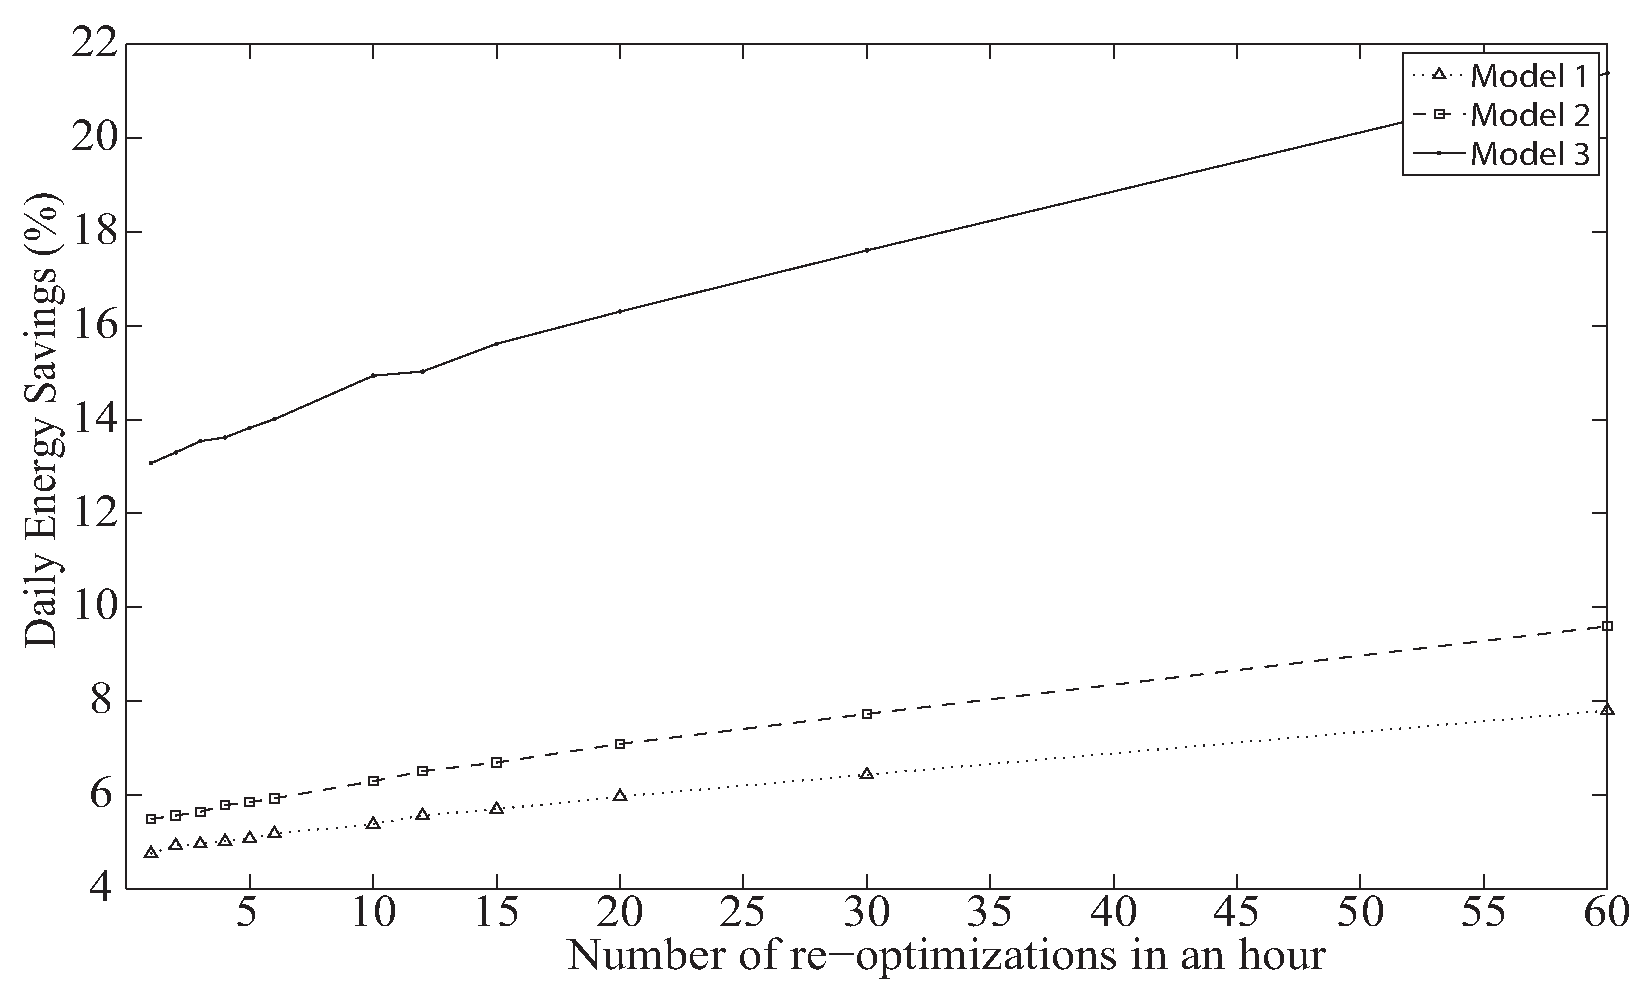
\includegraphics[width=0.8\textwidth]{pics/ilyas5a.eps}
\label{fig:results2}
}
\subfigure[]{
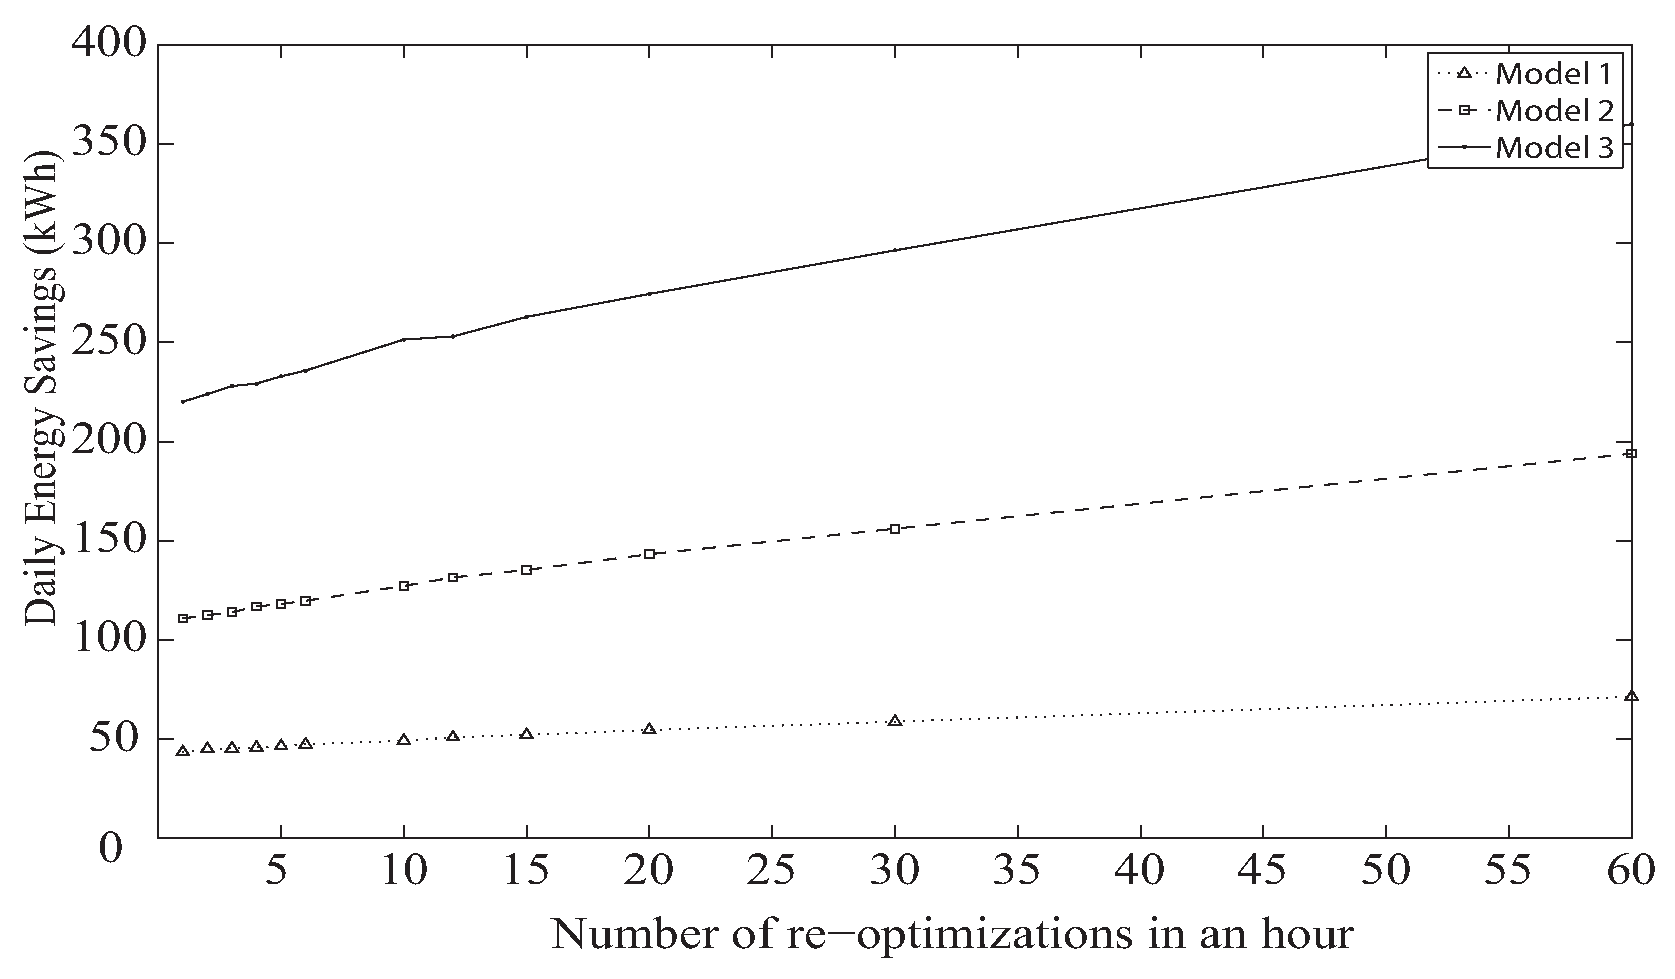
\includegraphics[width=0.8\textwidth]{pics/ilyas5b.eps}
\label{fig:results4}
}
\caption{(a) Percent reduction in energy consumption vs re-optimization interval, (b) Reduction in energy consumption vs re-optimization interval}
\label{fig:results24}
\end{figure}


To \textit{compare} the three BTS models in terms of energy saving potential, we also present the absolute reduction in energy consumption for the three BTS models in Figure~\ref{fig:results4}. We see the same linear trend along with the same relative order of the three models in terms of amount of saved energy, as in Figure~\ref{fig:results2}.

Re-optimizing at an interval less than the mean call duration should offer greater savings than a less frequent re-optimization, because the former regime is able to optimally assign BTSs to most of the calls at least once. This is confirmed in our results. For instance, the gain in energy savings for Model 1 BTS when going from a 60 minutes inter-optimization interval to 30 minutes gains an energy saving of only 0.0506\,kWh per minute, while decreasing the inter-optimization interval from 2 minutes to 1 minute gains 12.5421\,kWh.

Let us now interpret what these results mean physically in terms of ecological impact. If we extrapolate our results, the total energy saving for Pakistan are projected to be $60.72$\,MWh, $156.84$\,MWh and $301.61$\,MWh daily, respectively, according to the three BTS models. These savings in energy are significant, especially for small and developing countries. Since network deployments and traffic patterns are similar in different countries, we also expect that similar savings should be achievable in many other countries as well.

In the above extrapolation, we have assumed that the same amount of energy saving would be applicable in rural as well as urban settings. While this may not necessarily be true because the deployments are sparse in rural settings, resulting in reduced potential to save energy by means of call hand-off to neighboring sites, the potential to save energy merely by BTS power-saving should be higher in a rural setting because traffic loads are typically lower.

\subsection{Multi-state BTS}
\label{subsec:results2}
In our experimental results discussed so far, we have observed that going from a 6+6+6 configuration to a 2+2+2 configuration can save a significant amount of energy. Intuition suggests that going to a finer granularity of resource pruning should enable greater energy savings. We now present two cases that are different from the configuration considered so far. In the first case, we consider the ability to (de)activate TRXs in pairs, i.e., a site may be in one of three configurations at a given time: 6+6+6, 4+4+4 or 2+2+2. In the second case, we consider the ability to (de)activate each TRX on a site independently.

In this scenario, we conducted simulation experiments where a re-optimization was performed every six minutes using all three BTS models. The results of these experiments are given in Table~\ref{tab:granularityresults}. For all three BTS models, we see that going from a 2-state model to a 3-state model gives a relatively small increase in energy savings. However, when all TRXs may be independently controlled, we get a significant improvement in energy savings.

\begin{table}
\centering
\begin{tabular}{|c|c|c|c|}
\hline
Granularity & BTS Model 1 & BTS Model 2 & BTS Model 3\\
\hline 2-State & 5.38\% & 6.29\% &  14.94\% \\
\hline 3-State & 6.81\% & 7.73\% &  18.62\% \\
\hline $r$-State & 8.70\% & 9.65\% &  23.37\% \\
\hline
\end{tabular}
\vspace{+0.1in}
\caption{Percentage electricity savings for different granularity of resource pruning}
\label{tab:granularityresults}
\end{table}

\subsection{Performance of heuristic algorithm}
\label{subsec:heur1-results}
\begin{figure}
\centering
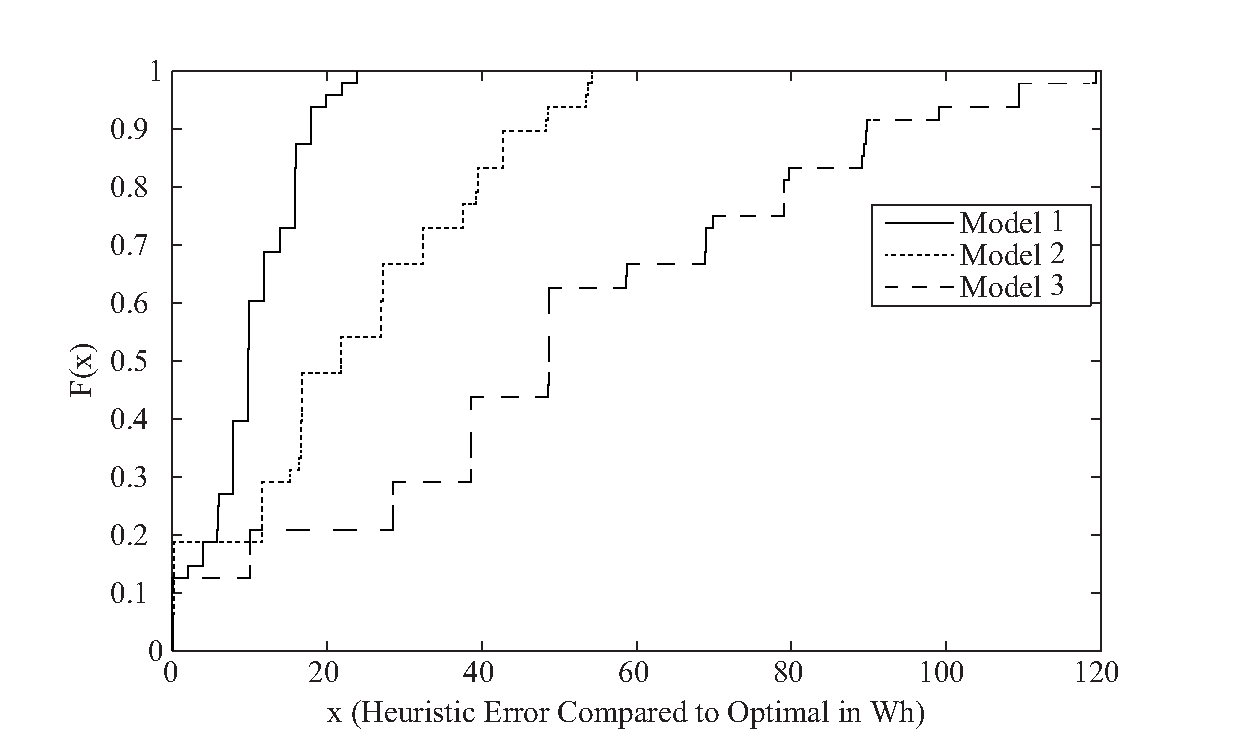
\includegraphics[width=0.8\textwidth]{pics/ilyas6.eps}
\caption{Empirical CDF of the difference between the cost offered by our heuristic compared to the optimal}
\label{fig:results5}
\end{figure}

We also ran experiments for each BTS model in which the electricity cost for the optimal as well as the heuristic algorithm (Algorithm 1) was computed. We assessed the performance of our heuristic by computing the difference (error) in the electricity cost of the two solutions. For statistical significance, we computed the error in our heuristic relative to the optimal solution over 48 different experiment runs for each BTS model. The resulting CDF of the heuristic error (in Wh) is plotted in Figure~\ref{fig:results5}. We can see in Figure~\ref{fig:results5} that our heuristic algorithm 1 is quite close to the optimal solution most of the time, especially for the Model 1 and Model 2 BTS. For Model 3 BTS, although the error is comparatively larger, but since the amount of savings with the optimal solution is quite high (Figure~\ref{fig:results2}), the heuristic will still result in significant energy savings.

\subsection{Sensitivity to the value of $\epsilon$}
\label{subsec:results3}
If the value of $\epsilon$ in our optimization is set too aggressively, a BTS may oscillate at times between low power and high power states rapidly due to short time scale traffic variations. Such state oscillations may be undesirable and to avoid these, the value of $\epsilon$ must be set at a safe value. Furthermore, if $\epsilon$ is set too aggressively, a BTS placed in low-power mode would be operating very close to its \textit{new} and lower traffic capacity. If several calls arrive in a short time window, the BSC may not have sufficient time to bring the BTS back into high-power mode and, thus, some calls may be blocked. However, if $\epsilon$ is set too conservatively, the energy savings would be smaller.

We carried out experiments to assess the impact of the value of $\epsilon$ on the energy savings achievable through RED-BL. For this purpose, we fixed the inter-optimization interval at 6 minutes and carried out RED-BL optimizations for all three BTS models. Furthermore, we considered a two-state BTS model, i.e., a BTS may be placed in either a 6+6+6 or a 2+2+2 configuration. The range of possible values for epsilon were 5, 10, 15 and 25. Since the traffic capacity of a 2+2+2 BTS is 44\footnote{The capacity of the 2+2+2 BTS is 3$\times$2$\times$8 = 48, but 4 channels were reserved by the operator for control and broadcast channels.}, any larger value for $\epsilon$ did not make sense. Figure~\ref{fig:case2:results6} shows the results. As expected, the percentage savings deplete almost linearly with increasing values of $\epsilon$.

\begin{figure}
\centering
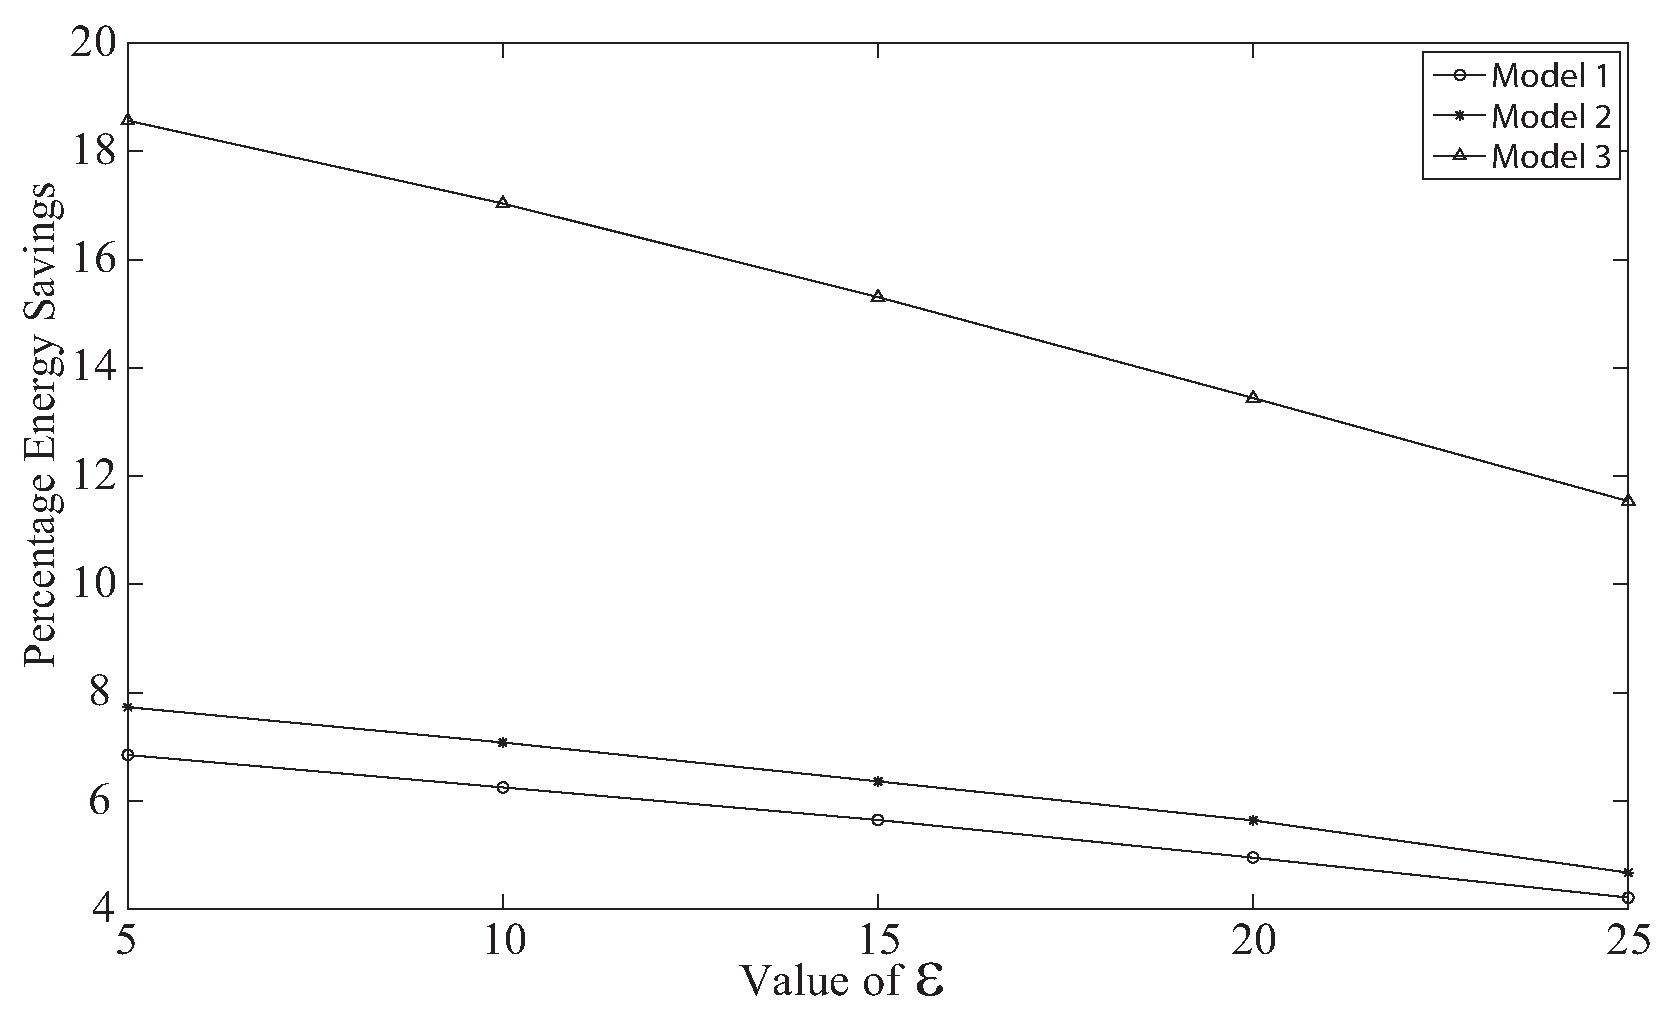
\includegraphics[width=0.8\textwidth]{pics/ilyas7.eps}
\caption{The percentage energy savings for all three BTS models considered vs the value of $\epsilon$, with a six minute inter-optimization interval}
\label{fig:case2:results6}
\end{figure}

\subsection{Increase in call blocking probability}
\label{subsec:callblock} A measure of a cellular network's grade of service (GoS) is the call blocking probability ($P_b$), given by the Erlang B formula~\cite{rappaport}. The Erlang B formula is:

$P_b = \frac{\frac{E^C}{C!}}{\sum_{k=0}^C\frac{E^k}{k!}}$

Here, $E$ is the traffic intensity in Erlang and $C$ is the number of identical resources that are available to serve the traffic. According to this formula, if the offered traffic remains the same, but some serving resources, i.e., TRXs are turned off, the call blocking probability may increase. This makes intuitive sense because given a fixed call load, a new arriving call is more likely to find all TRXs busy if the number of active TRXs is reduced.

We calculated the increase in call blocking probability, averaged over all BTSs and over the day, due to periodic optimization of the network's resources, compared to the default assignment of calls with no TRX deactivation. It turned out that more frequent re-optimization resulted in a greater increase in call blocking probability.  

The increase in call blocking probability with the amount of energy savings (kWh) is plotted in Figure~\ref{fig:results25} for all three BTS models. Similarly, the increase in call blocking probability as a function of percentage energy savings is plotted in Figure~\ref{fig:results26} for all three BTS models. For all the plots, the actual data points are plotted using the plus symbols, the linear fit and quadratic fit based on least squared errors are plotted using the solid black line and the dashed black line respectively. The linear and quadratic polynomials polynomials that best fit the increase in call blocking probability as a function of amount and percentage of daily energy savings are given in Tables~\ref{tab:blockpoly1} and~\ref{tab:blockpoly2}, respectively.

In all cases, a linear polynomial based on least squared error minimization fits the data quite well. However, the connotation in the low-savings region are unreasonable. As an example, for model 1 BTS, as shown in Figure~\ref{fig:results7.1}, the linear polynomial fit implies a reduction in call blocking probability when saving around 40 kWh compared to the default network operation. This does not make sense because turning off some TRXs to save power should result in an increase in call blocking probability. A quadratic fit to the data, however, is reasonable in all cases.

\begin{table}
\centering
\begin{tabular}{|c|c|}
\hline
BTS Model & Increase in call blocking probability as a function of \\
\ & amount of daily energy savings (kWh)\\
\hline Model 1 & Linear fit: $0.006888 x - 0.2816$\\
\ & Quadratic fit: $0.0001178 x^2 - 0.006524 x + 0.08914$\\
\hline Model 2 & Linear fit: $0.002262x - 0.2286$\\
\ & Quadratic fit: $0.00001297 x^2 - 0.001623 x + 0.05131$\\ 
\hline Model 3 & Linear fit: $0.001352x - 0.2766$ \\
\ & Quadratic fit: $0.000004627 x^2 - 0.001295 x + 0.09101$\\
\hline
\end{tabular}
\vspace{+0.1in}
\caption{Polynomial fits of increase in call blocking probability to amount of daily energy savings}
\label{tab:blockpoly1}
\end{table}

\begin{table}
\centering
\begin{tabular}{|c|c|}
\hline
BTS Model & Increase in call blocking probability as a function of \\
\ & percentage of daily energy savings\\
\hline Model 1 & Linear fit: $0.06368 x - 0.2835$\\
\ & Quadratic fit: $0.008113 x^2 -0.03747 x + 0.02244$\\
\hline Model 2 & Linear fit: $0.0457x - 0.2285$\\
\ & Quadratic fit: $0.005285x^2 -0.03266 x + 0.05084$\\ 
\hline Model 3 & Linear fit: $0.02276x - 0.2766$\\
\ & Quadratic fit: $0.001315 x^2 -0.02193 x +0.09201$ \\
\hline
\end{tabular}
\vspace{+0.1in}
\caption{Polynomial fits of increase in call blocking probability to percentage of daily energy savings}
\label{tab:blockpoly2}
\end{table}


\begin{figure}
\centering
\subfigure[]{
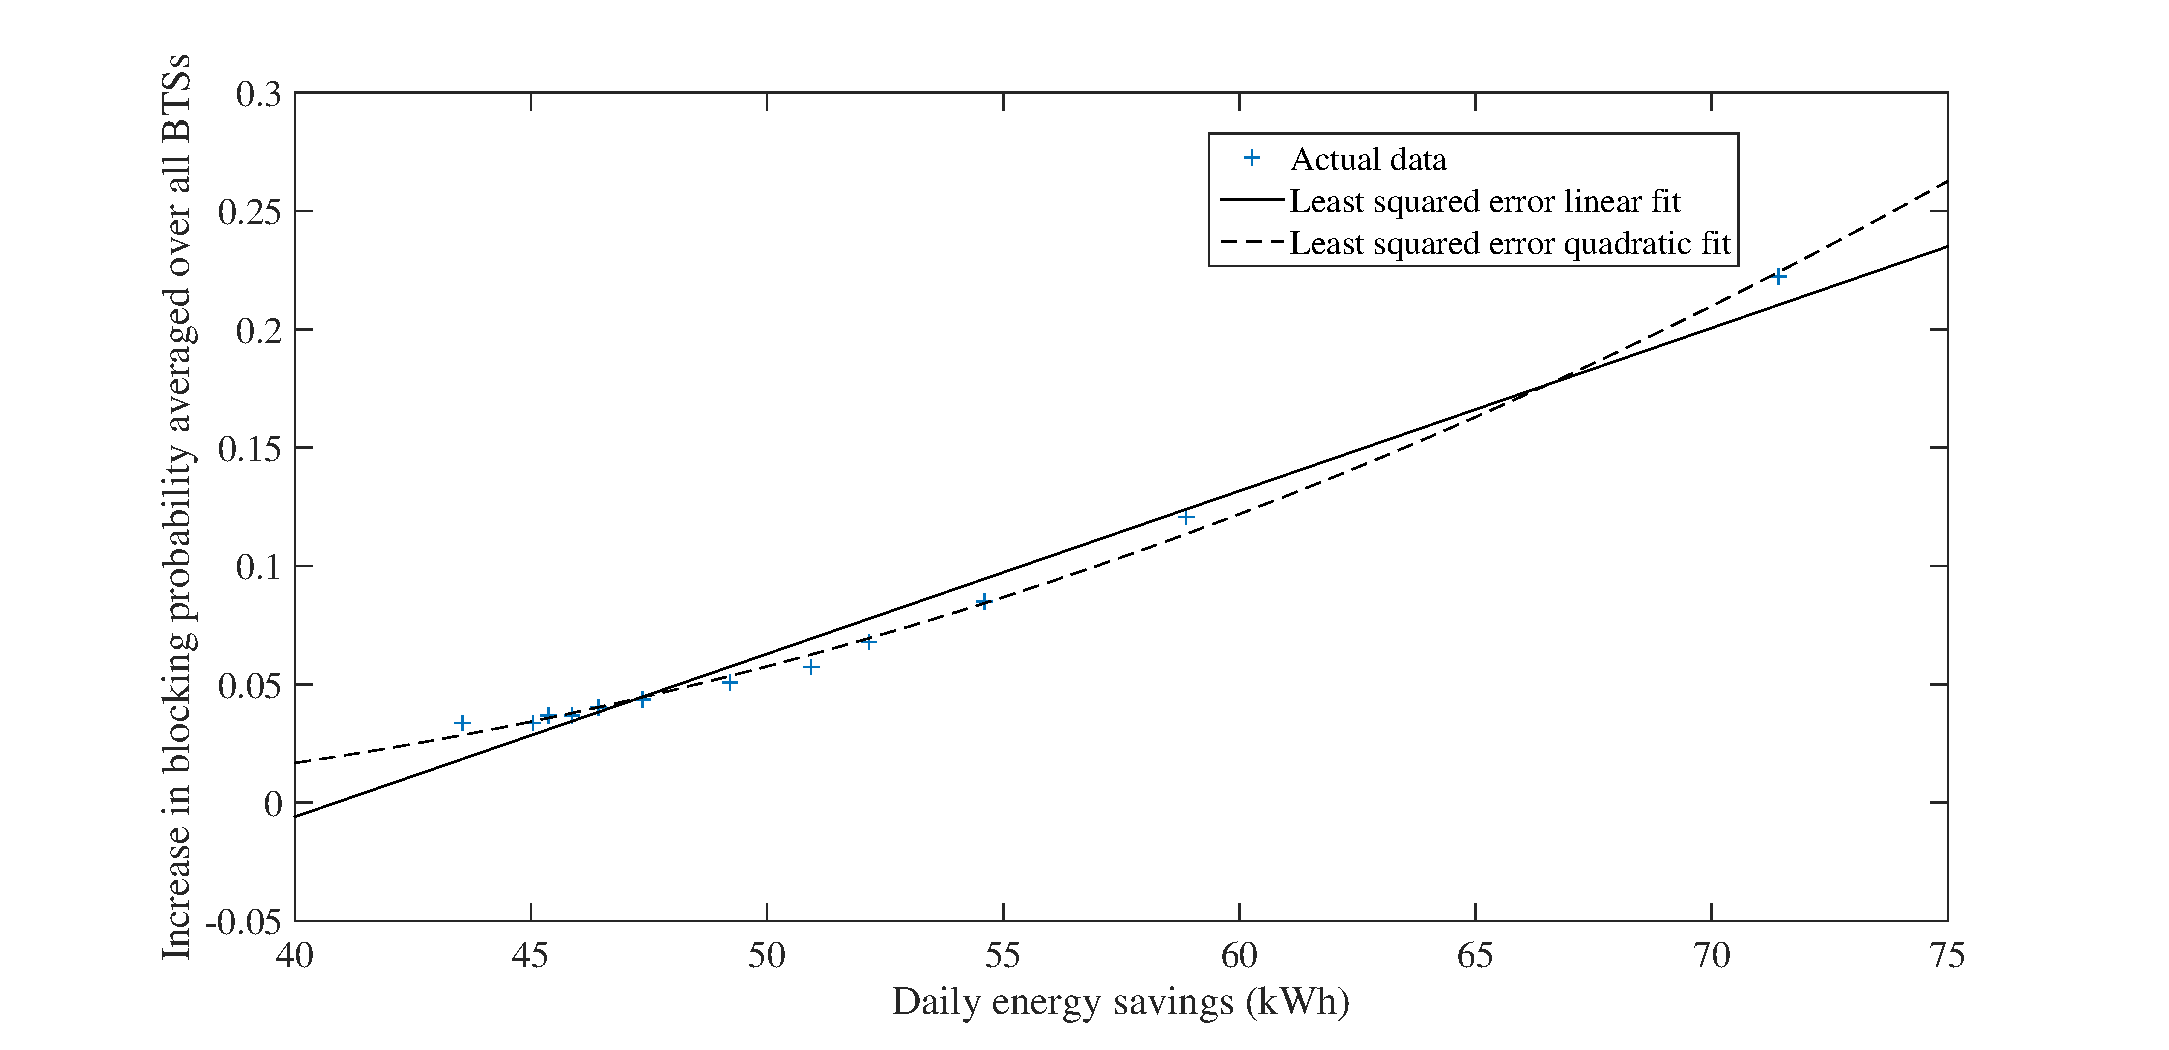
\includegraphics[width=0.8\textwidth]{pics/1.SavingvsBlockingProbIncrease.eps}
\label{fig:results7.1}
}
\subfigure[]{
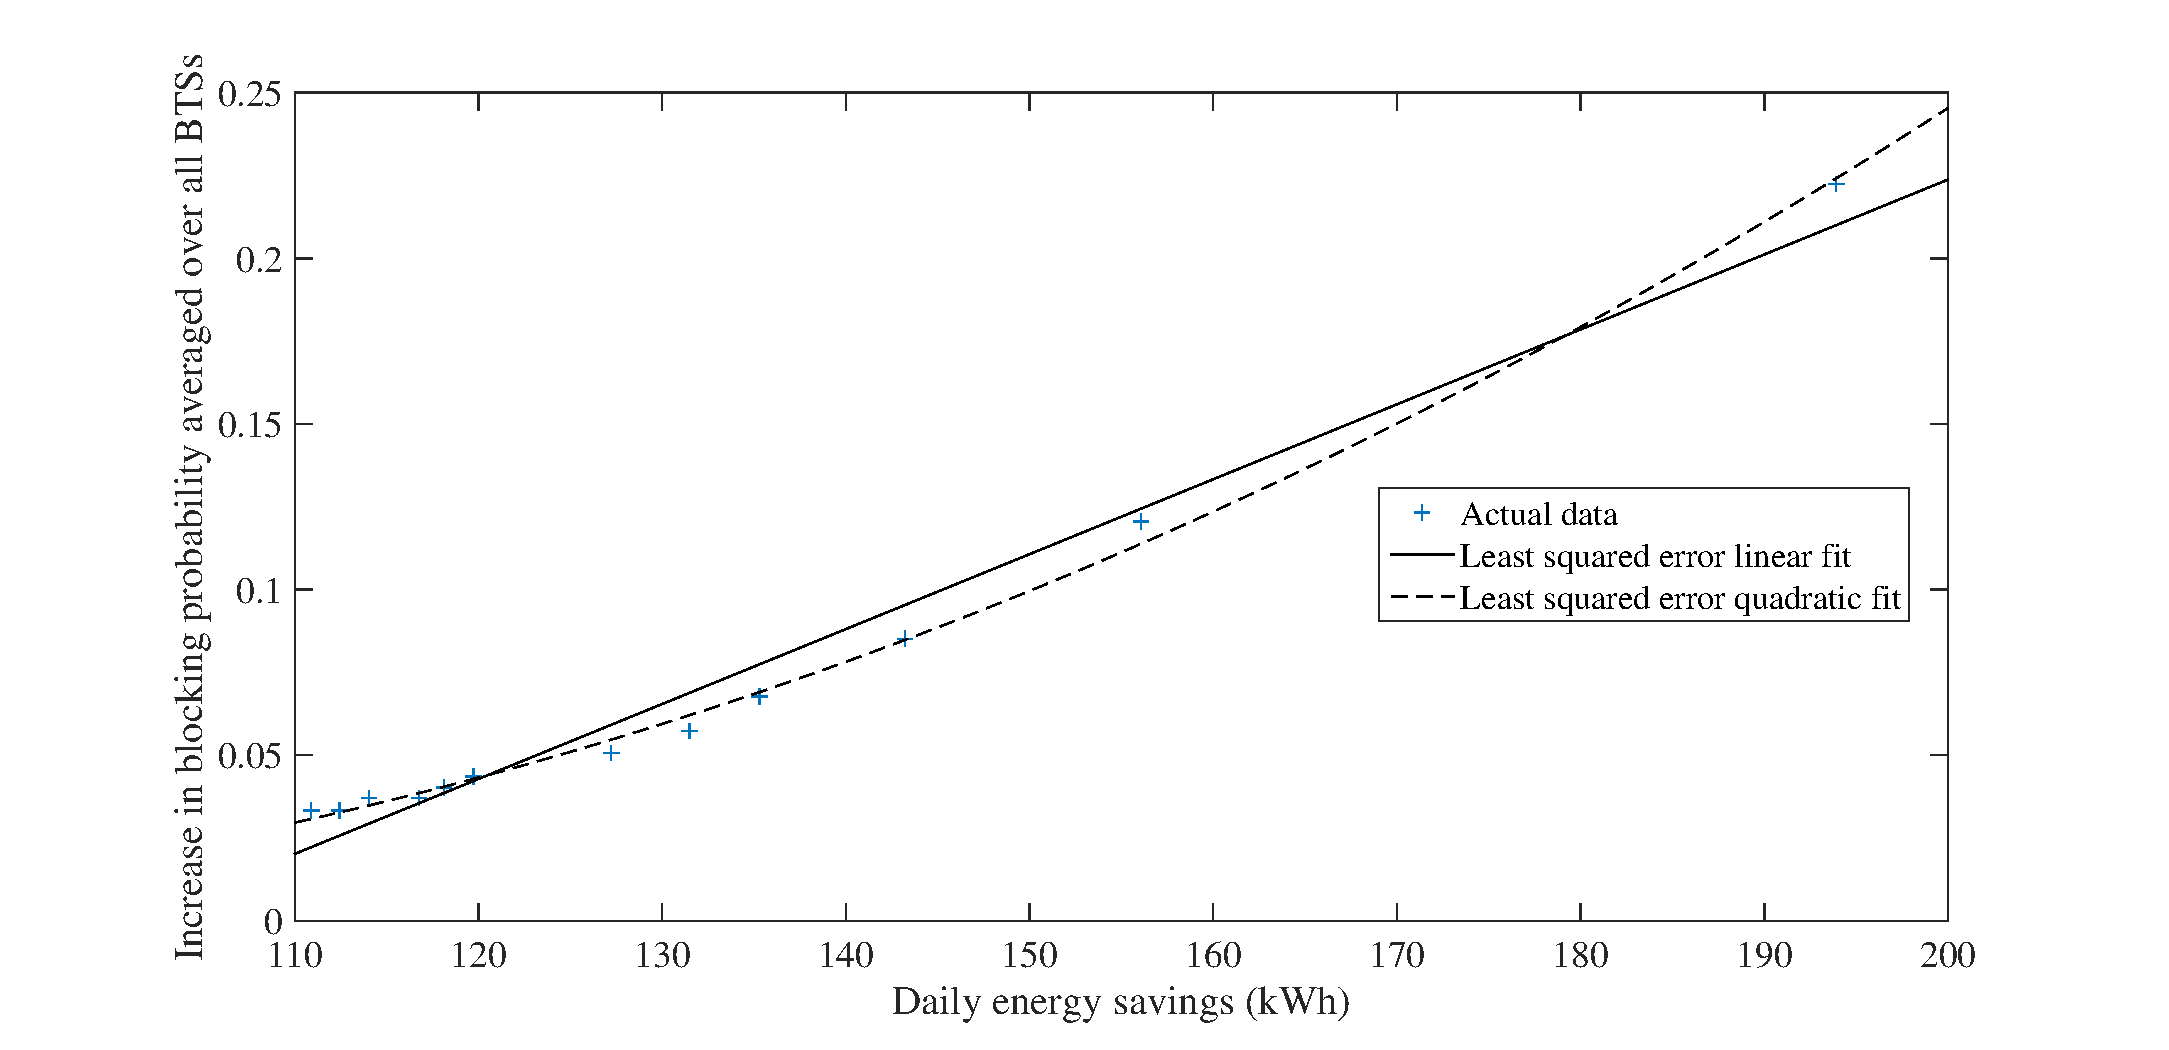
\includegraphics[width=0.8\textwidth]{pics/2.SavingvsBlockingProbIncrease.eps}
\label{fig:results7.2}
}
\subfigure[]{
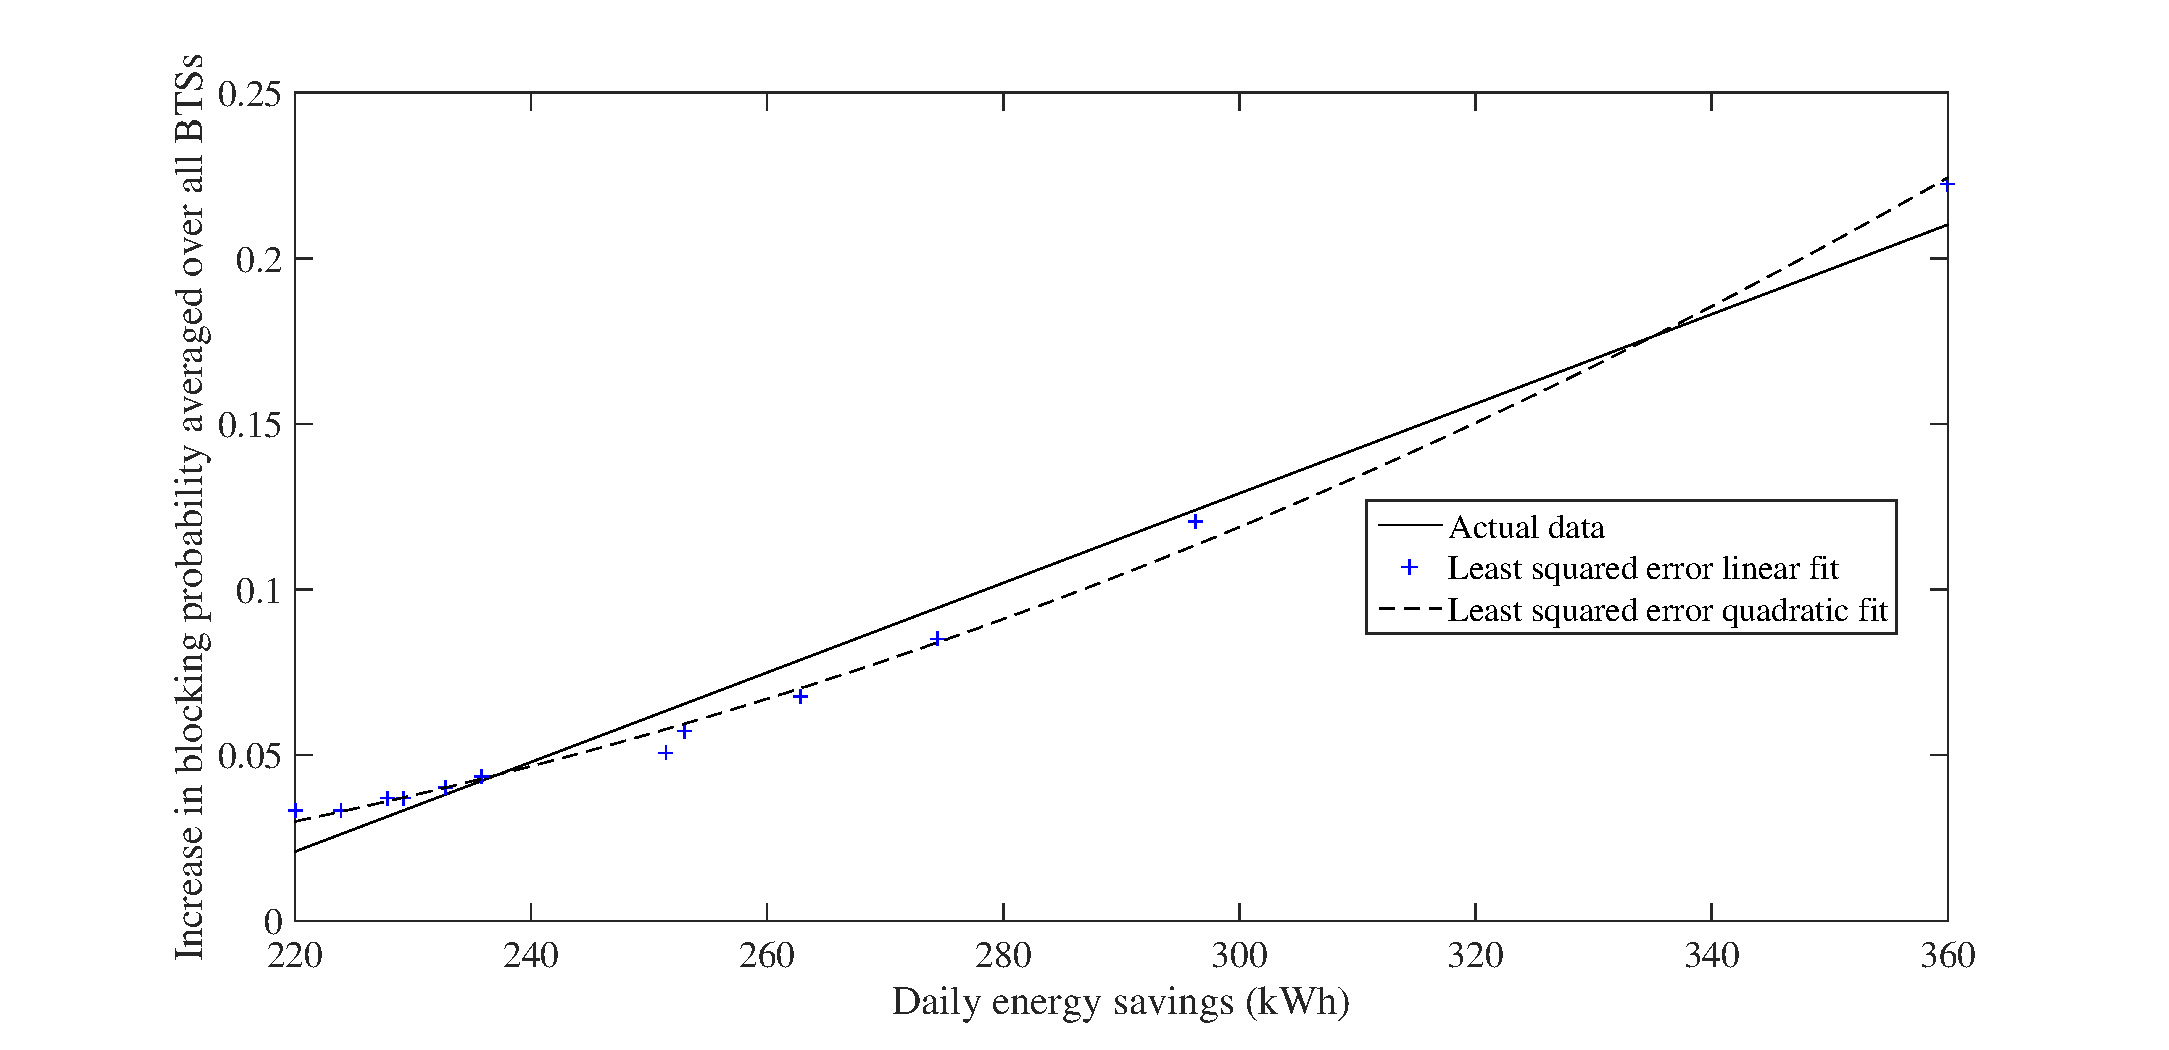
\includegraphics[width=0.8\textwidth]{pics/3.SavingvsBlockingProbIncrease.eps}
\label{fig:results7.3}
}
\caption{Increase in call blocking probability, averaged over all BTSs versus the amount of daily energy savings in kWh for (a) BTS model 1 (b) BTS model 2 and (c) BTS model 3}
\label{fig:results25}
\end{figure}

\begin{figure}
\centering
\subfigure[]{
\includegraphics[width=0.8\textwidth]{pics/1.percSavingvsBlockingProbIncrease.eps}
\label{fig:results7.4}
}
\subfigure[]{
\includegraphics[width=0.8\textwidth]{pics/2.percSavingvsBlockingProbIncrease.eps}
\label{fig:results7.5}
}
\subfigure[]{
\includegraphics[width=0.8\textwidth]{pics/3.percSavingvsBlockingProbIncrease.eps}
\label{fig:results7.6}
}
\caption{Increase in call blocking probability, averaged over all BTSs versus the percentage reduction in energy consumption for (a) BTS model 1 (b) BTS model 2 and (c) BTS model 3}
\label{fig:results26}
\end{figure}

\section{Summary}
\label{sec:discuss:case2} In this chapter, we have seen an application of RED-BL to cellular networks. The nature of cellular networks is different compared to geo-diverse data centers (considered in the previous chapter) in the following ways:

\begin{itemize}
\item The workload (calls) has limited geographic flexibility and may only be handled at a few candidate resources (BTSs)
\item There is no geo-diversity in electricity prices
\end{itemize}

For resource pruning and workload relocation, we utilized two features built in to currently deployed equipment in the form of BTS power savings and network-controlled call hand-off, respectively. Our simulation results show that jointly using workload relocation and resource pruning can bring in considerably higher gains in electricity savings compared to using resource pruning alone. Our results show the promising potential that RED-BL holds in greening current generation cellular networks. However, dynamic deactivation of TRXs results in an increase in call blocking probability. We find that the increase in call blocking probability may be predicted from the amount or percentage of daily energy savings using a quadratic polynomial. An operator can pick the maximum amount of targeted energy savings based on their grade of service budget. This can, in turn, be used to decide how frequently traffic and TRX re-optimization should be performed.